% Present the findings of your research. Provide a detailed 
% analysis of the performance of the various algorithms used 
% for weather prediction, including their accuracy, precision, 
% and recall rates.

% The results section of your thesis presents the findings of 
% your study. It should provide a clear and concise summary of 
% the data collected and analyzed, along with any statistical 
% tests or other methods used to analyze the data. Here are some 
% important elements to consider including in your results section:

% Overall, the results section of your thesis should provide a 
% clear and concise summary of your findings, along with any statistical 
% tests or other methods used to analyze the data. It should also provide 
% an interpretation of your findings and relate them back to your research 
% questions or hypotheses.
\section{Wyniki}

% Descriptive statistics: Provide descriptive statistics that 
% summarize the main characteristics of your data, such as means, 
% standard deviations, and frequency distributions.
\subsection{Statystyki}

\begin{figure}[H]
    \centering
    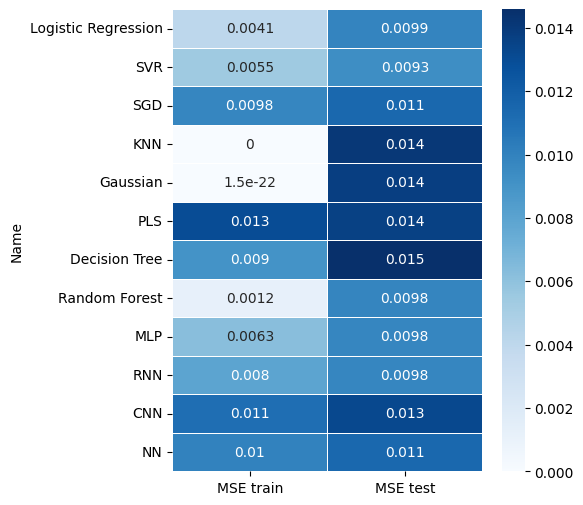
\includegraphics[width=\textwidth]{images/mse.png}
    \caption{}
    \label{mse}
\end{figure}

\begin{figure}[H]
    \centering
    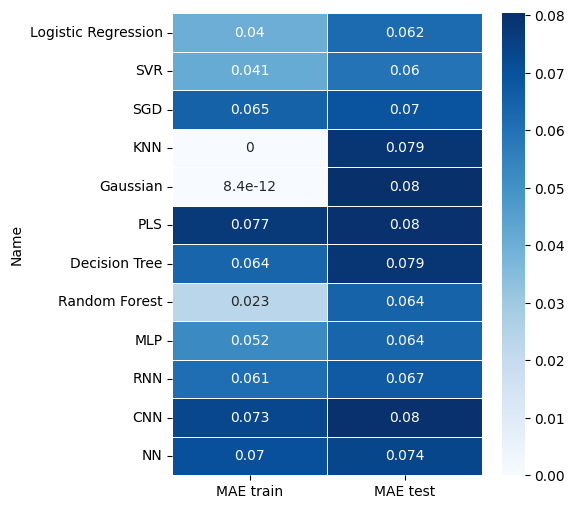
\includegraphics[width=\textwidth]{images/mae.png}
    \caption{}
    \label{mae}
\end{figure}

\begin{figure}[H]
    \centering
    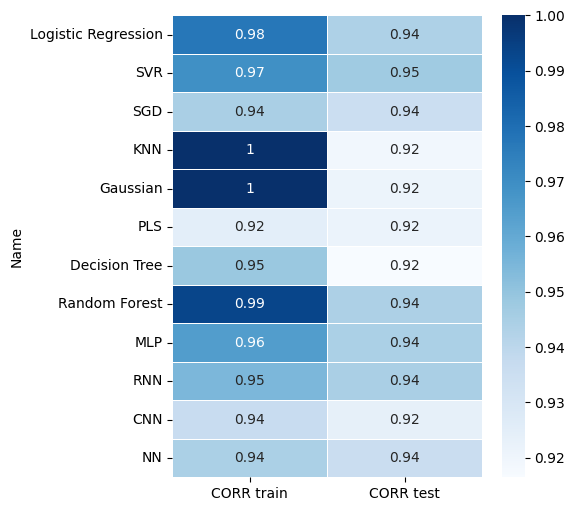
\includegraphics[width=\textwidth]{images/corr.png}
    \caption{}
    \label{corr}
\end{figure}

\begin{figure}[H]
    \centering
    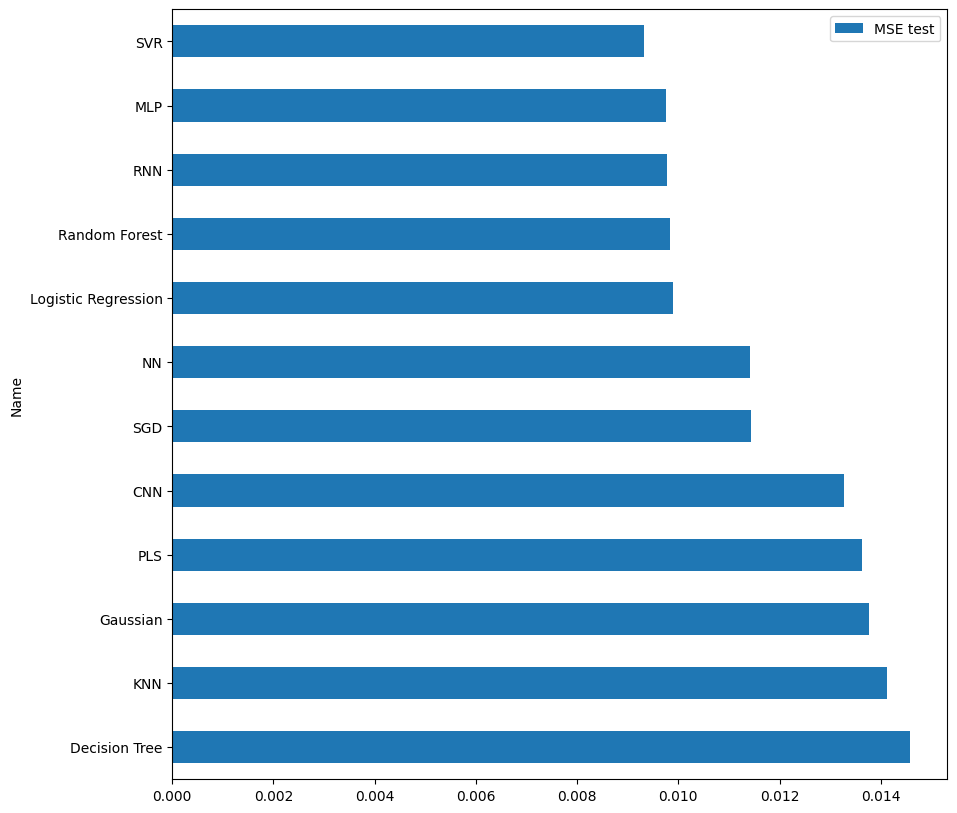
\includegraphics[width=\textwidth]{images/mse_ranking.png}
    \caption{}
    \label{mse-ranking}
\end{figure}

\begin{figure}[H]
    \centering
    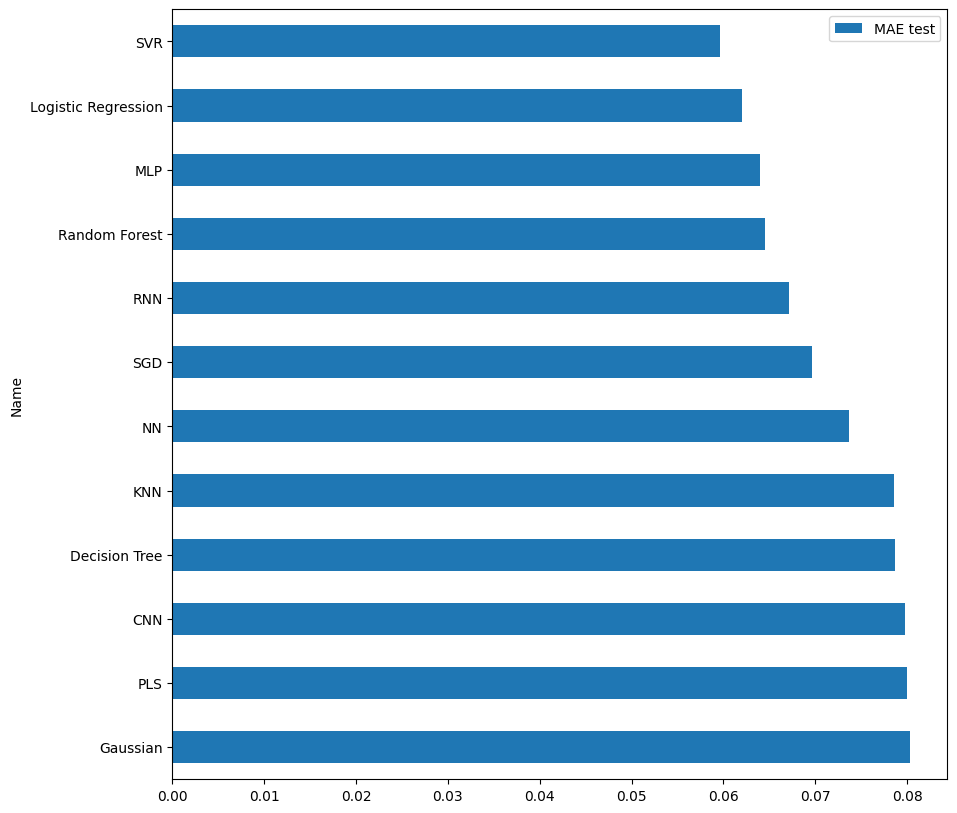
\includegraphics[width=\textwidth]{images/mae_ranking.png}
    \caption{}
    \label{mae-ranking}
\end{figure}

\begin{figure}[H]
    \centering
    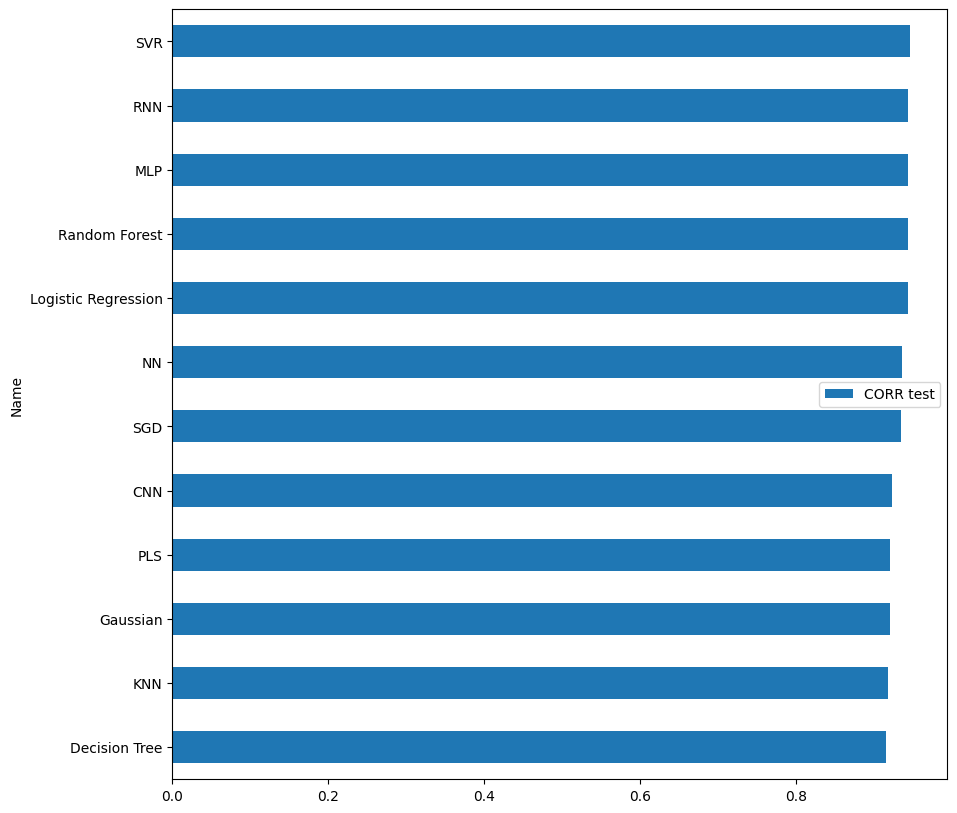
\includegraphics[width=\textwidth]{images/corr_ranking.png}
    \caption{}
    \label{corr-ranking}
\end{figure}

\begin{figure}[H]
    \centering
    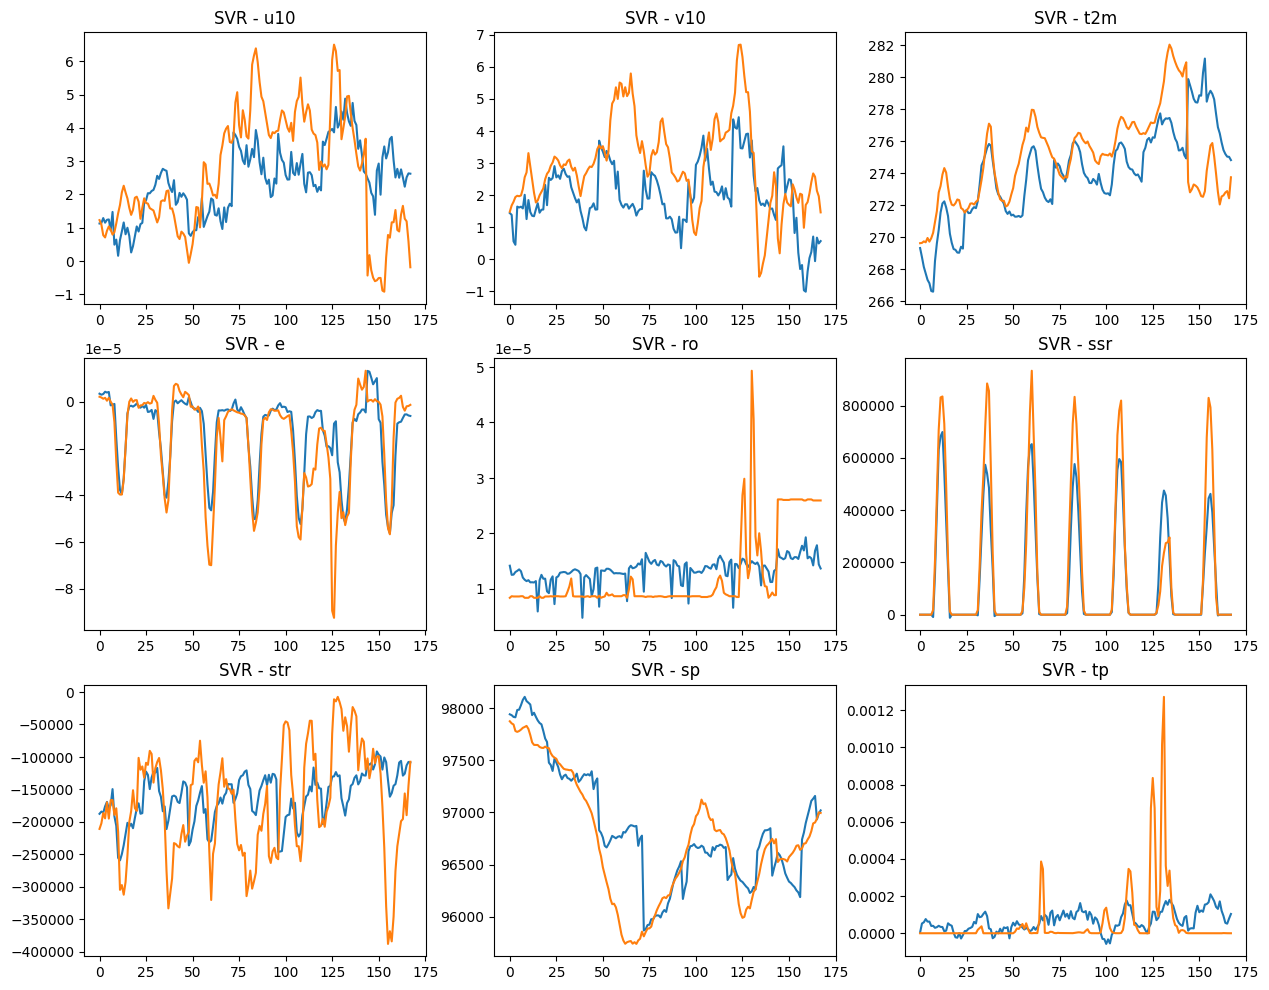
\includegraphics[width=\textwidth]{images/SVR_week.png}
    \caption{}
    \label{svr-week}
\end{figure}

\begin{figure}[H]
    \centering
    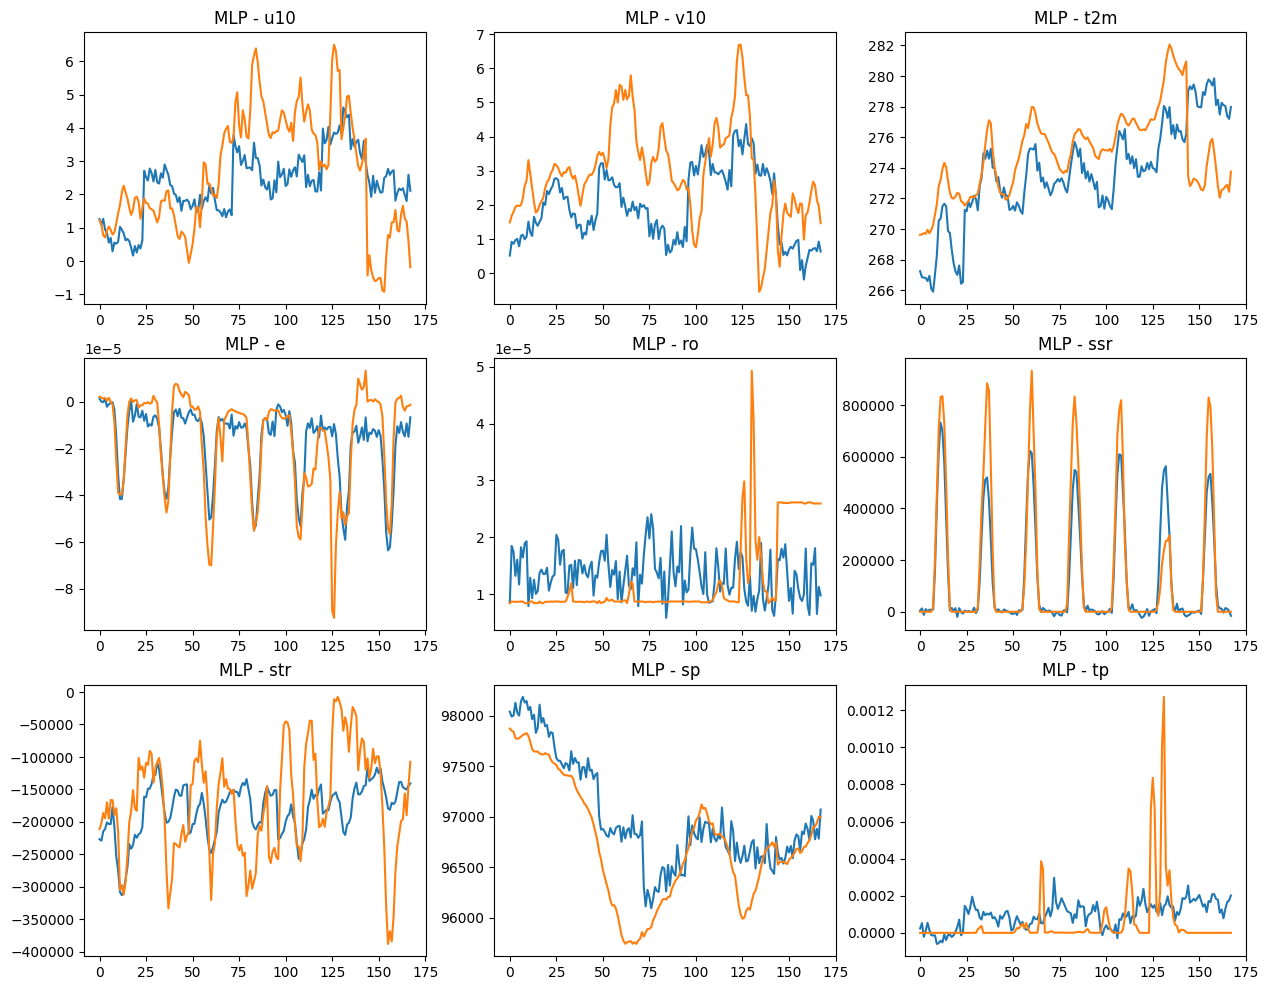
\includegraphics[width=\textwidth]{images/MLP_week.png}
    \caption{}
    \label{mlp-week}
\end{figure}

\begin{figure}[H]
    \centering
    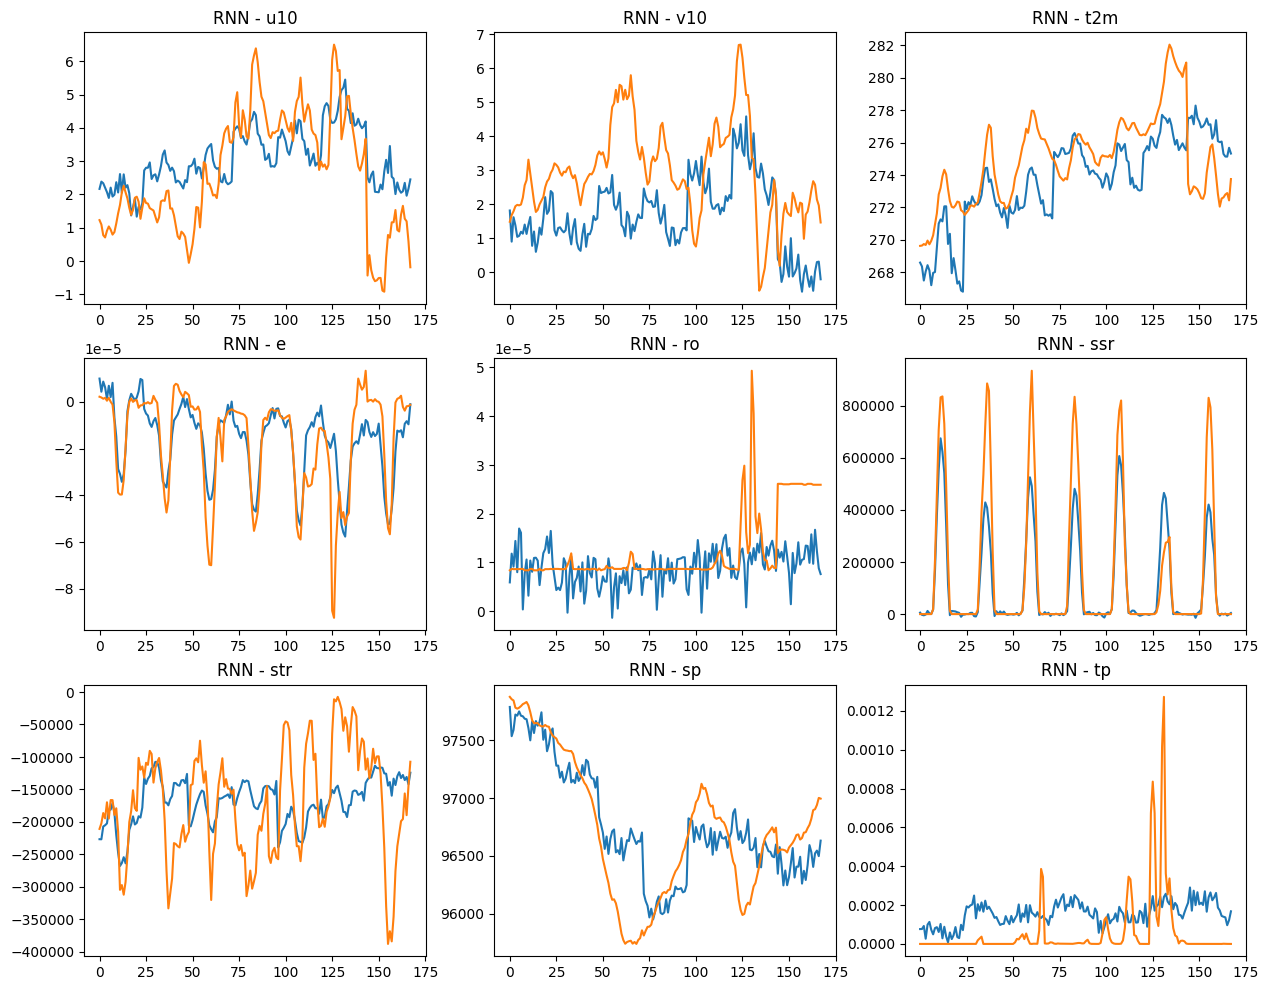
\includegraphics[width=\textwidth]{images/rnn_week.png}
    \caption{}
    \label{rnn-week}
\end{figure}

\begin{figure}[H]
    \centering
    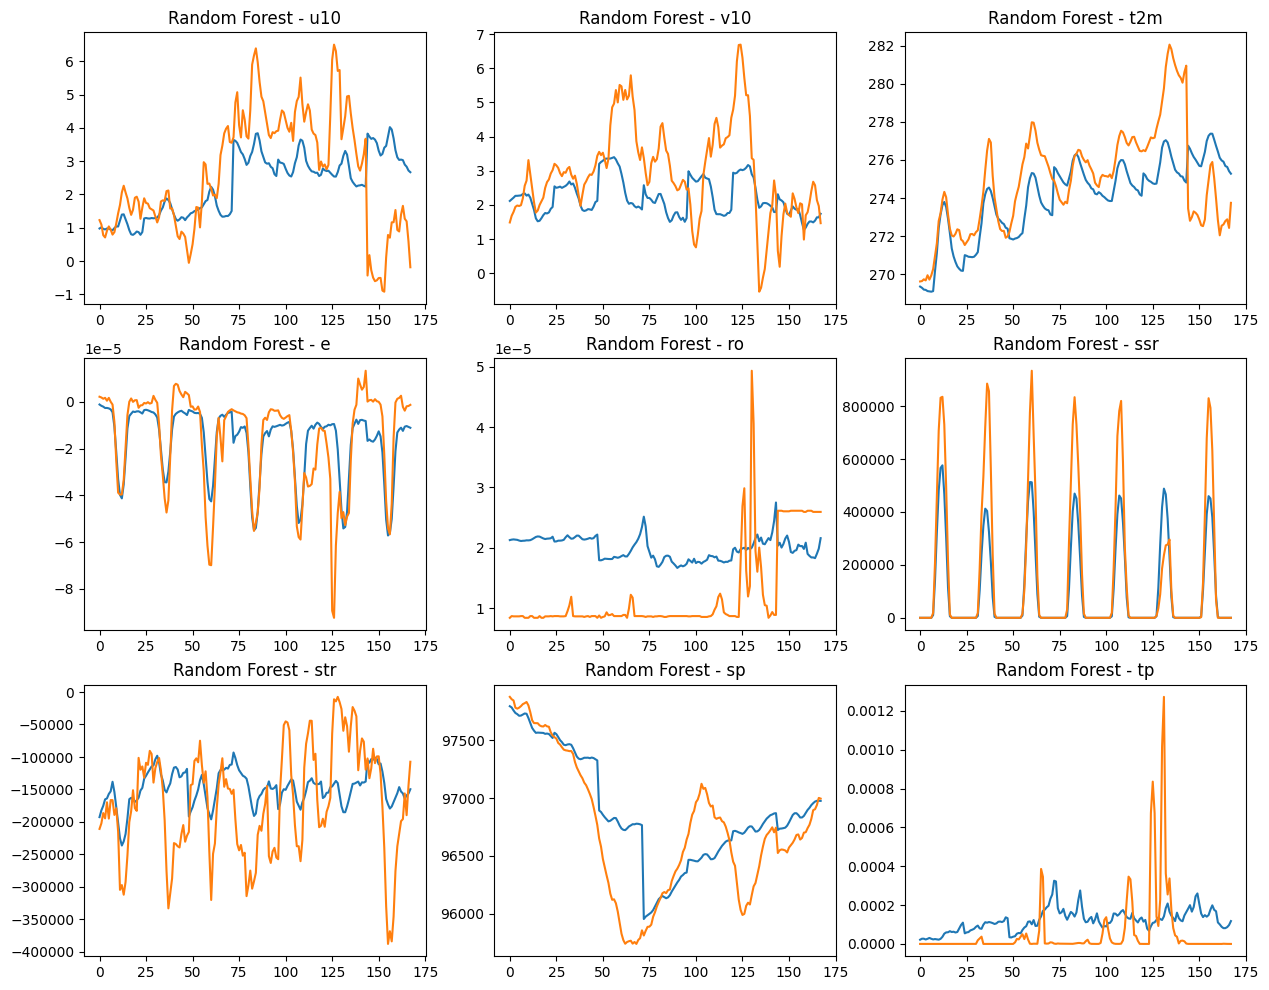
\includegraphics[width=\textwidth]{images/random_forest_week.png}
    \caption{}
    \label{forest-week}
\end{figure}

\begin{figure}[H]
    \centering
    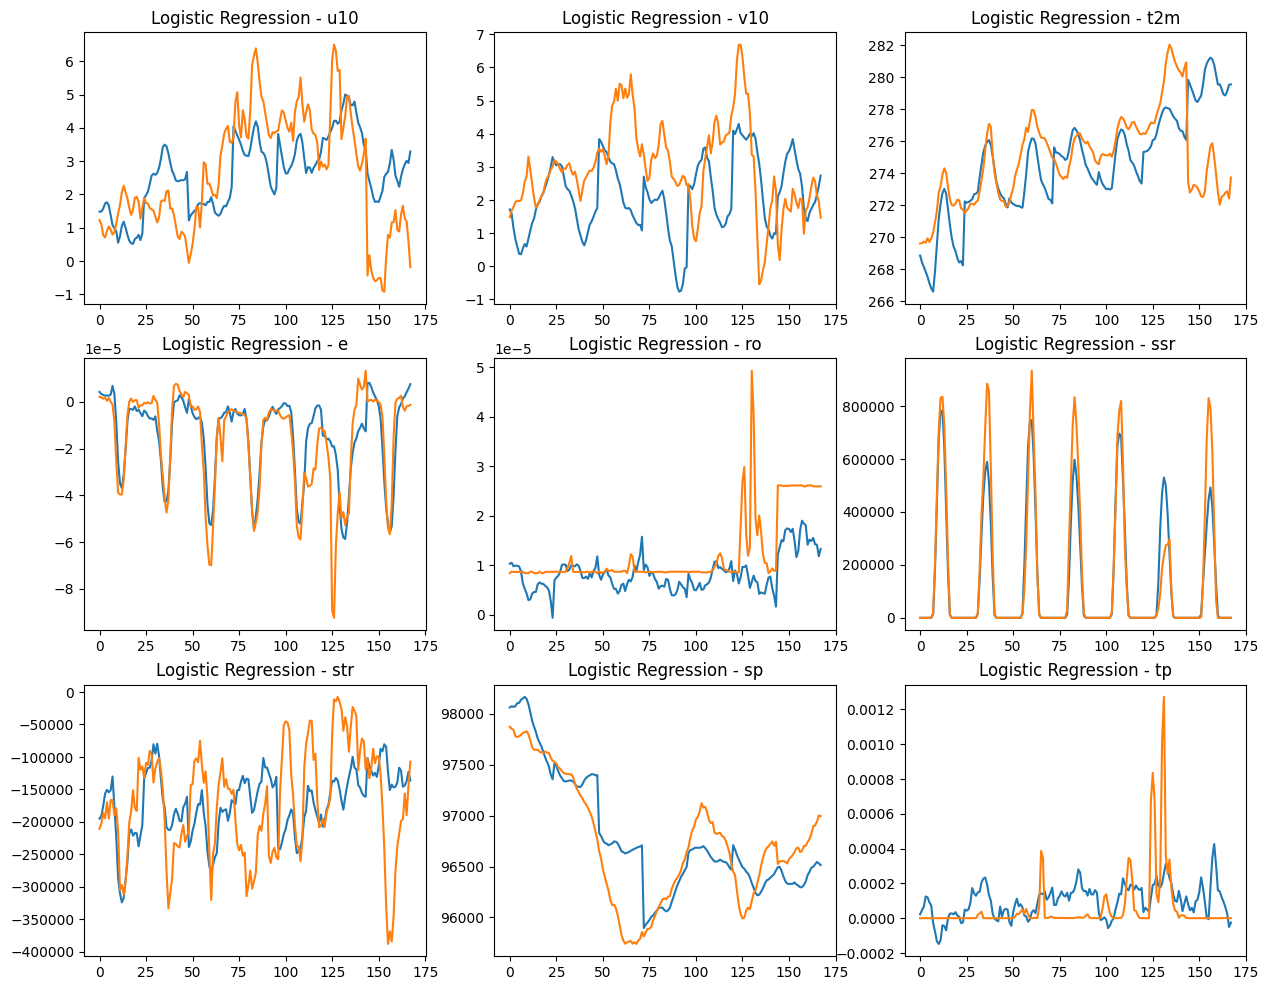
\includegraphics[width=\textwidth]{images/regression_week.png}
    \caption{}
    \label{regression-week}
\end{figure}

\begin{figure}[H]
    \centering
    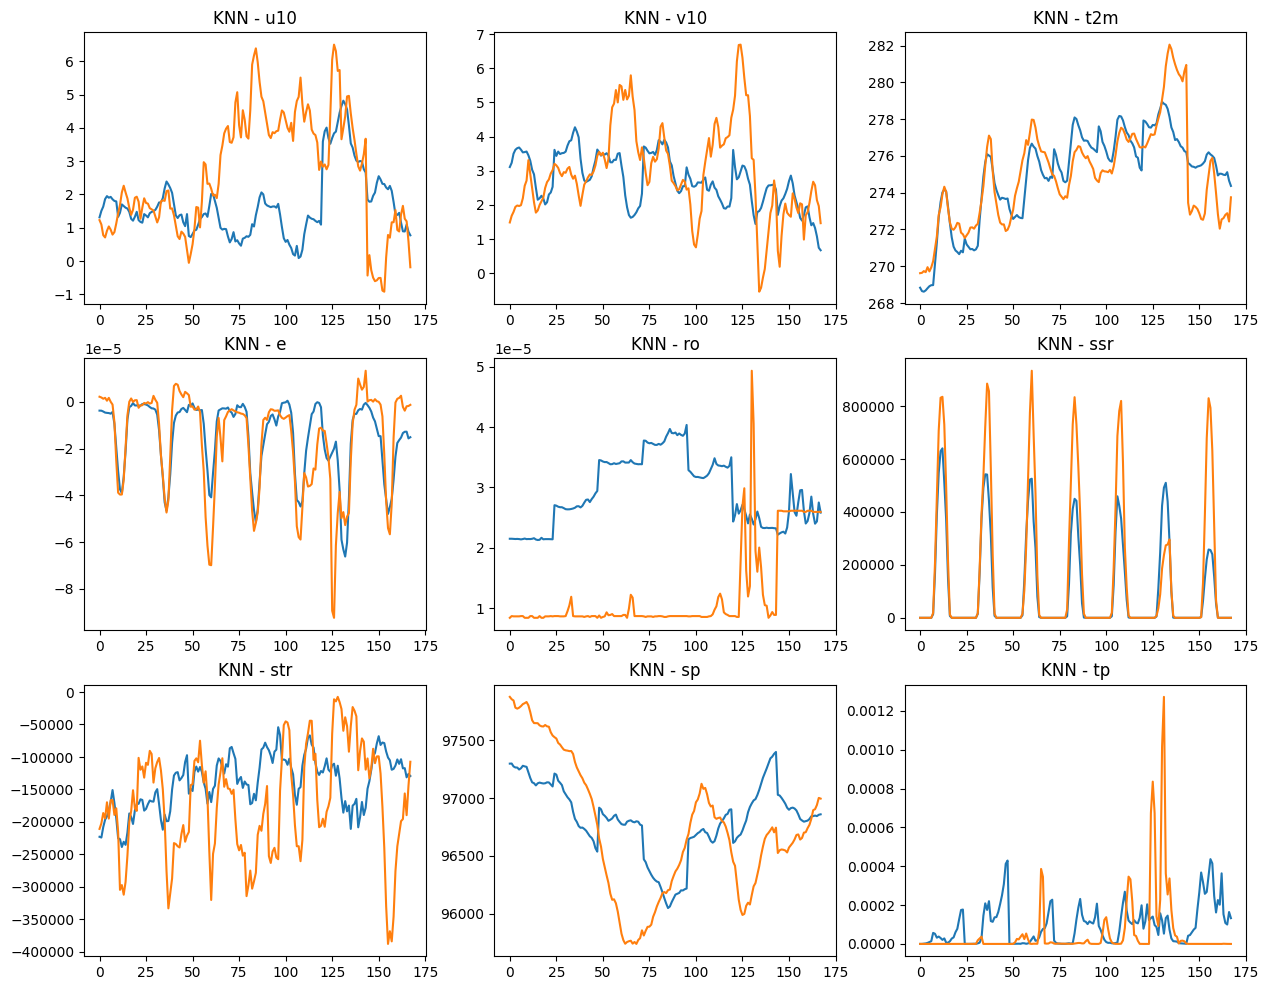
\includegraphics[width=\textwidth]{images/knn_week.png}
    \caption{}
    \label{knn-week}
\end{figure}

\begin{figure}[H]
    \centering
    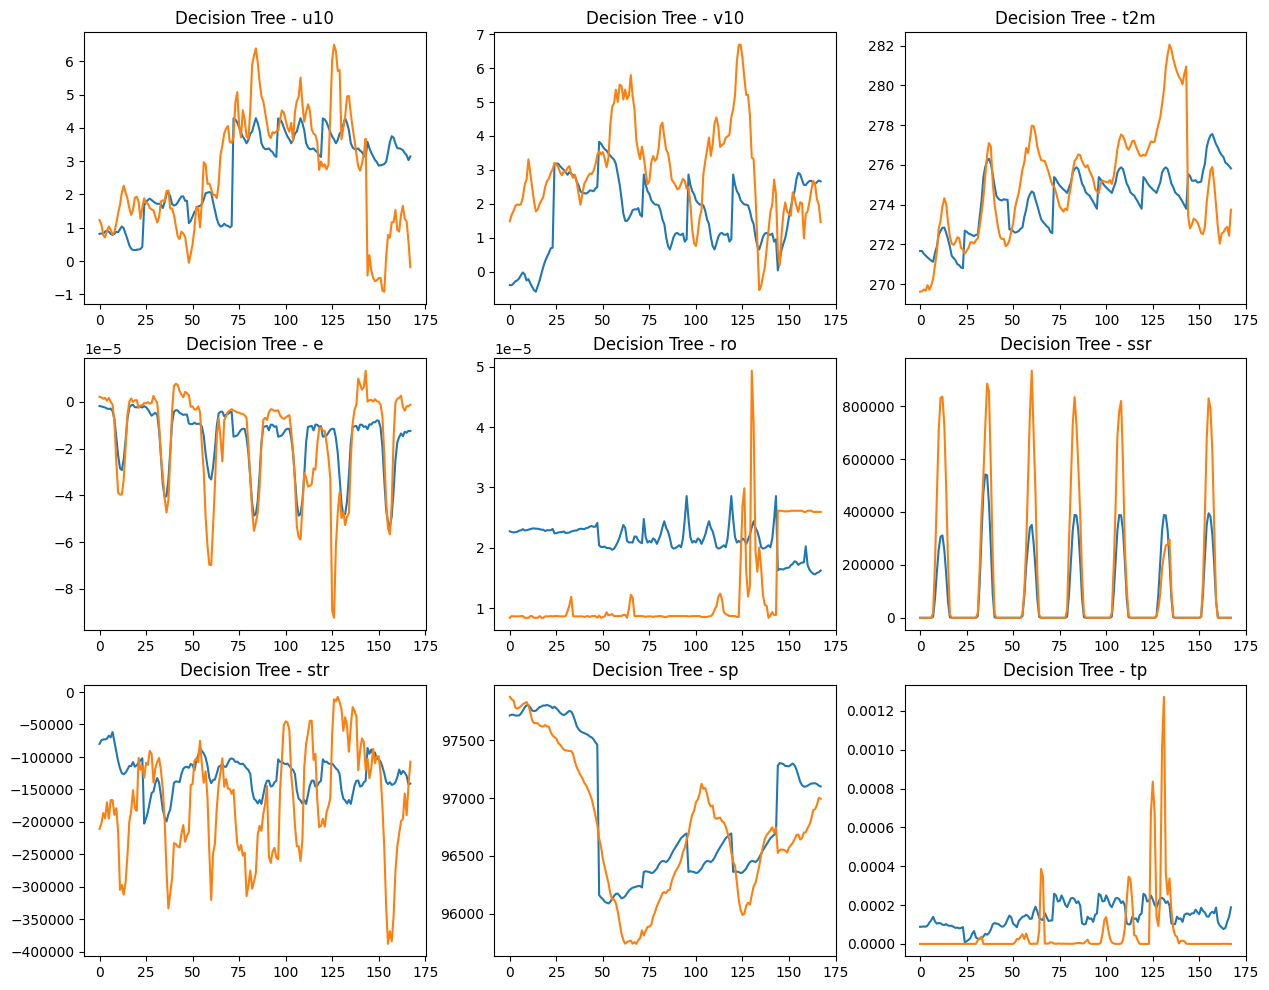
\includegraphics[width=\textwidth]{images/Decision_tree_week.png}
    \caption{}
    \label{tree-week}
\end{figure}

% Inferential statistics: Report the results of any inferential 
% statistical analyses that you conducted to test your research 
% hypotheses, such as t-tests, ANOVA, regression analysis, or 
% other statistical tests. Be sure to include the statistical 
% significance of the results and the effect sizes.
\subsection{Testy statystyczne}

\begin{figure}[H]
    \centering
    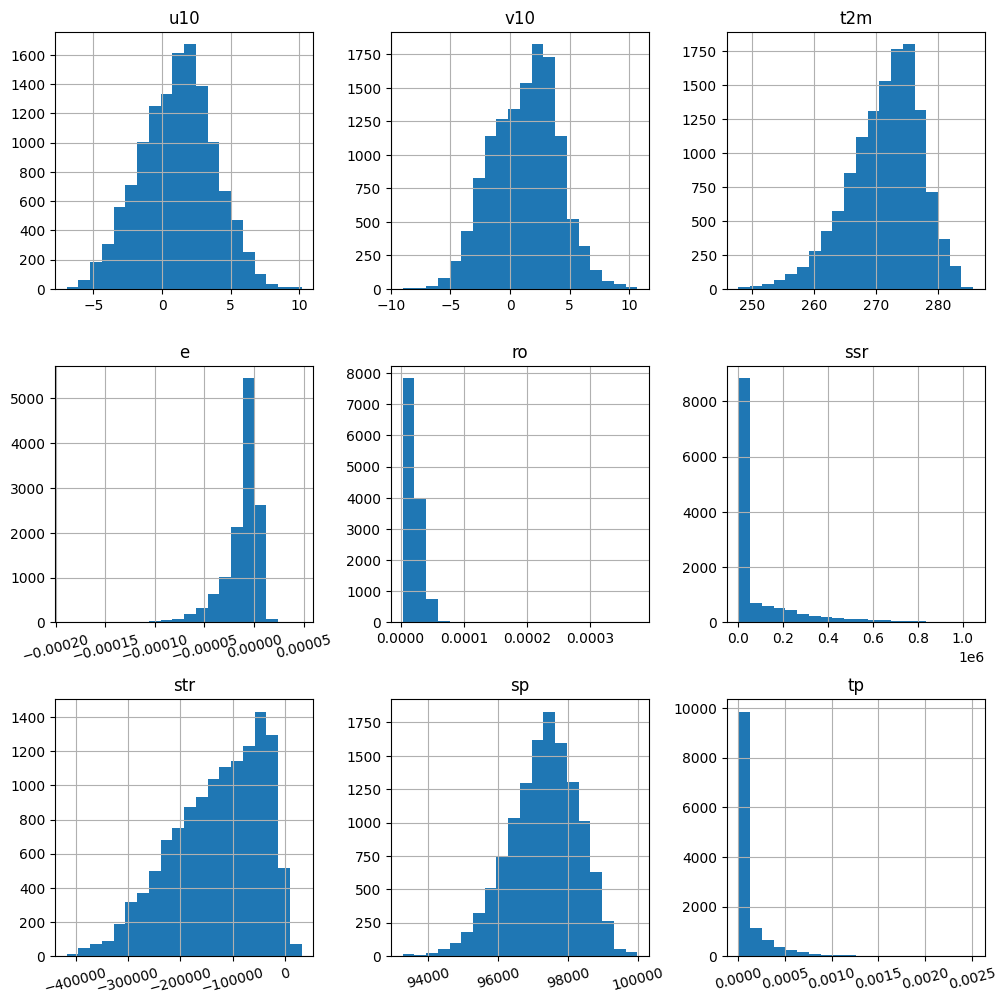
\includegraphics[width=\textwidth]{images/hist.png}
    \caption{}
    \label{real-hist}
\end{figure}

\begin{figure}[H]
    \centering
    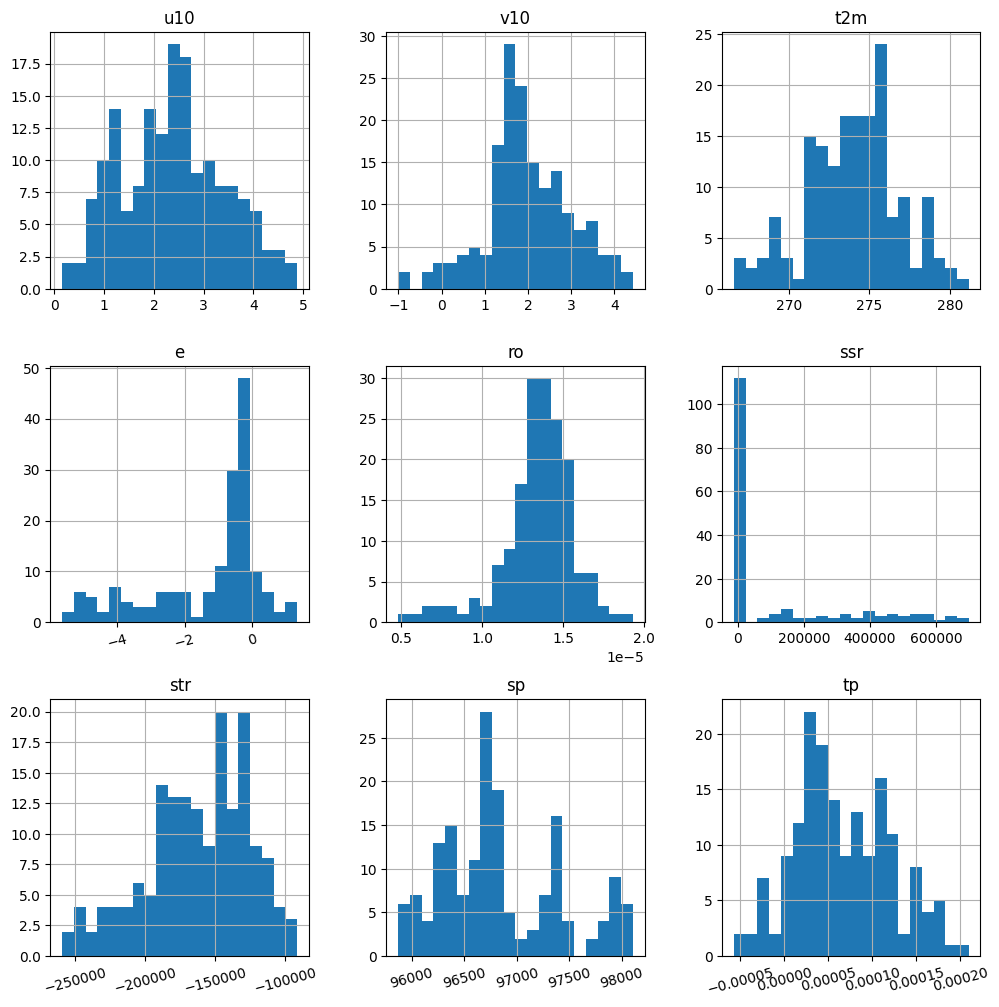
\includegraphics[width=\textwidth]{images/svr_hist.png}
    \caption{}
    \label{svr-hist}
\end{figure}

\begin{figure}[H]
    \centering
    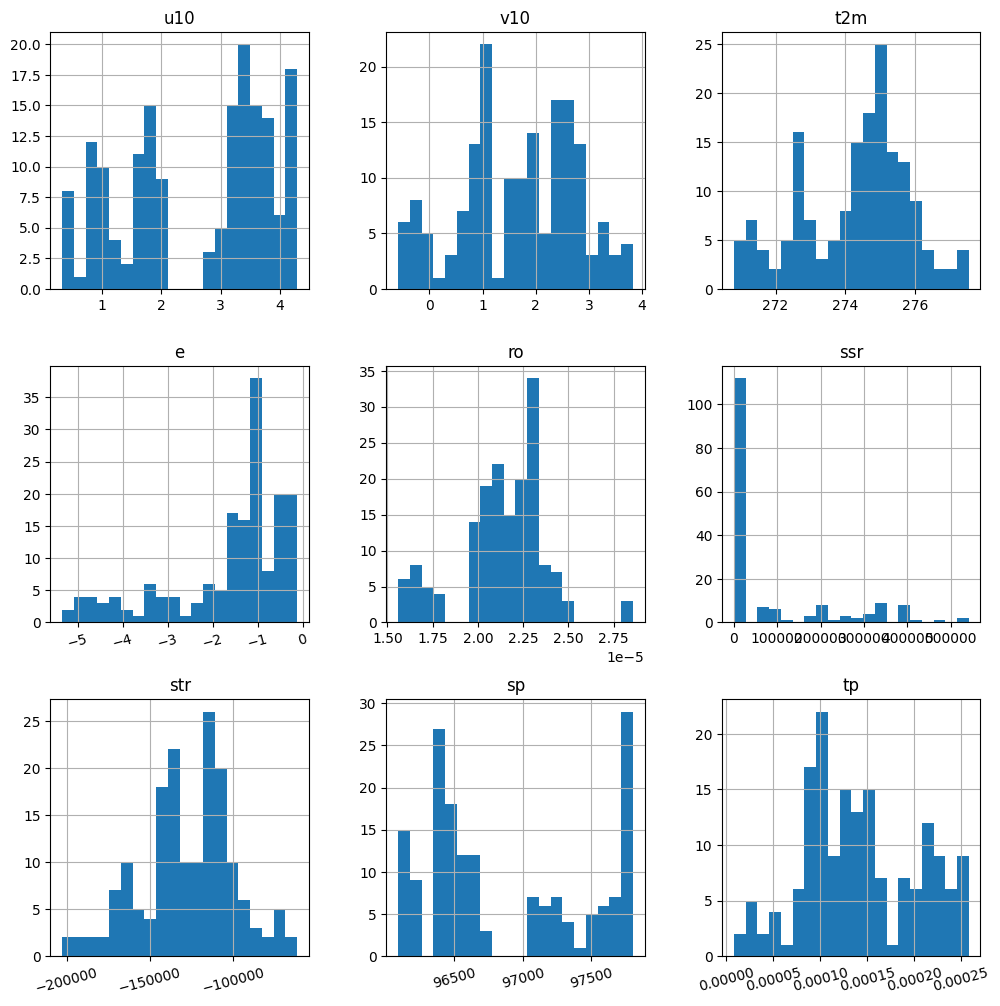
\includegraphics[width=\textwidth]{images/dt_hist.png}
    \caption{}
    \label{dt-hist}
\end{figure}



% Tables and figures: Present your data in tables and figures 
% that are clear, concise, and easy to read. Ensure that your 
% tables and figures are properly labeled and that they effectively 
% illustrate your findings.

% Subgroup analyses: Conduct subgroup analyses if relevant to 
% your research questions. For example, if you are comparing the 
% performance of different machine learning models, you might conduct 
% subgroup analyses based on the type of model used or the size of the training data.
\subsection{Porównanie modeli}

\begin{figure}[H]
    \centering
    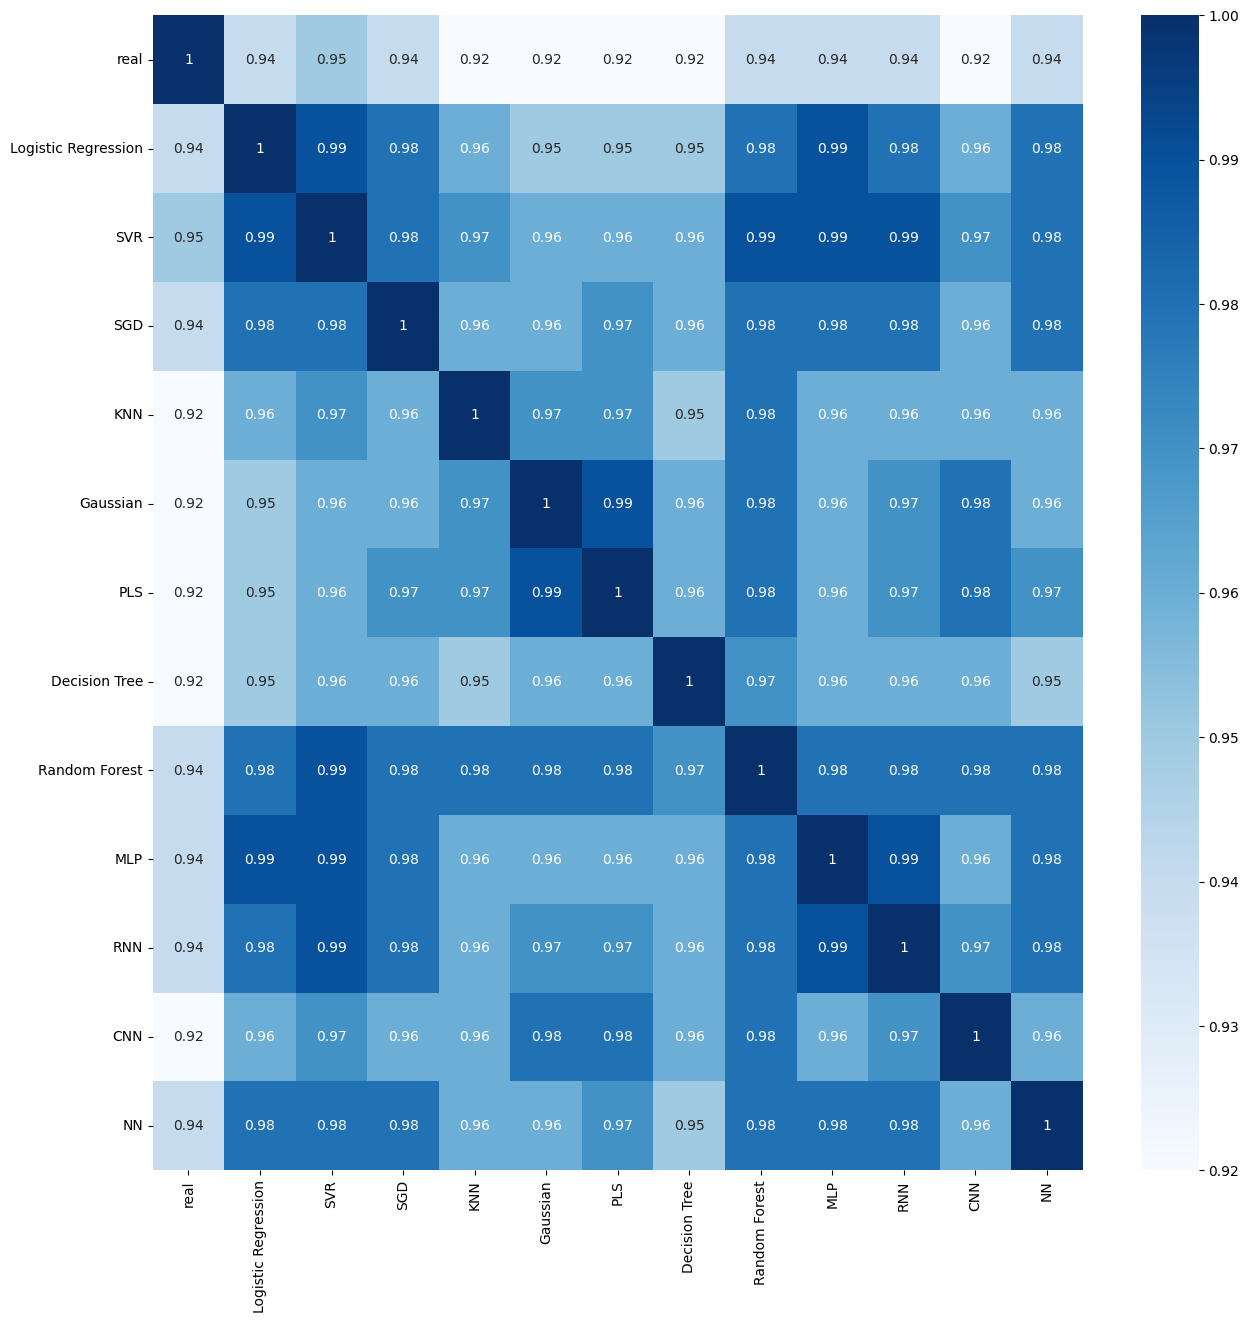
\includegraphics[width=\textwidth]{images/pred_corr.png}
    \caption{}
    \label{pred_corr}
\end{figure}

\begin{figure}[H]
    \centering
    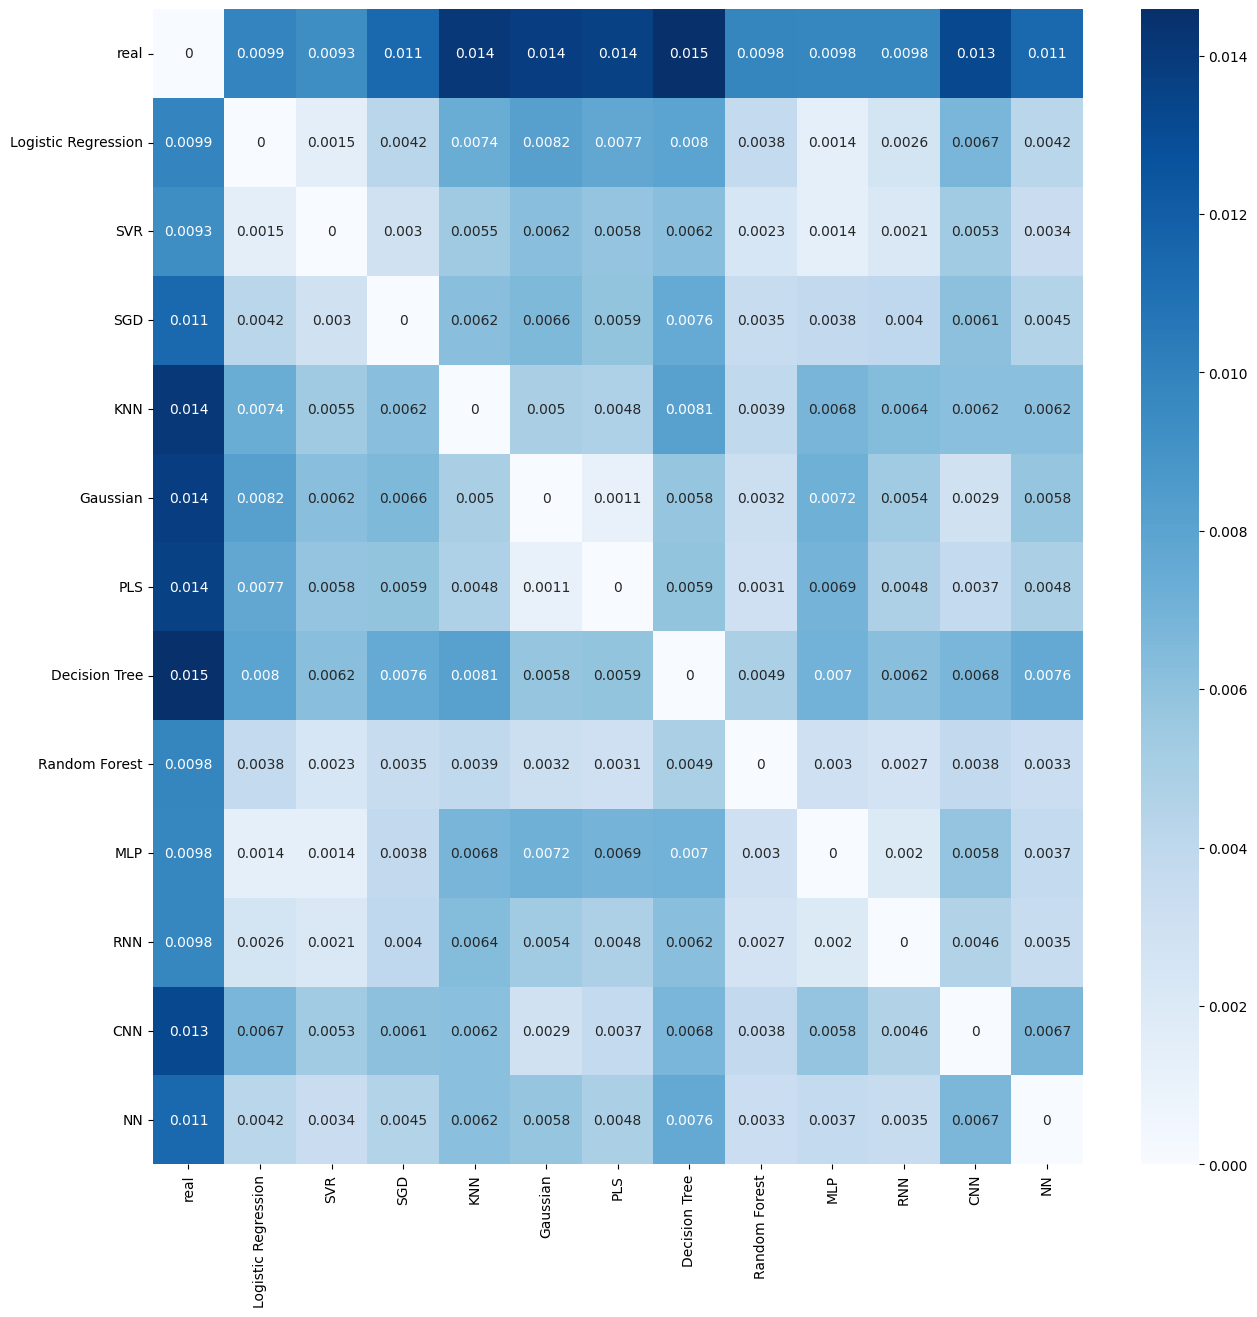
\includegraphics[width=\textwidth]{images/mse_matrix.png}
    \caption{}
    \label{mse-matrix}
\end{figure}

\begin{figure}[H]
    \centering
    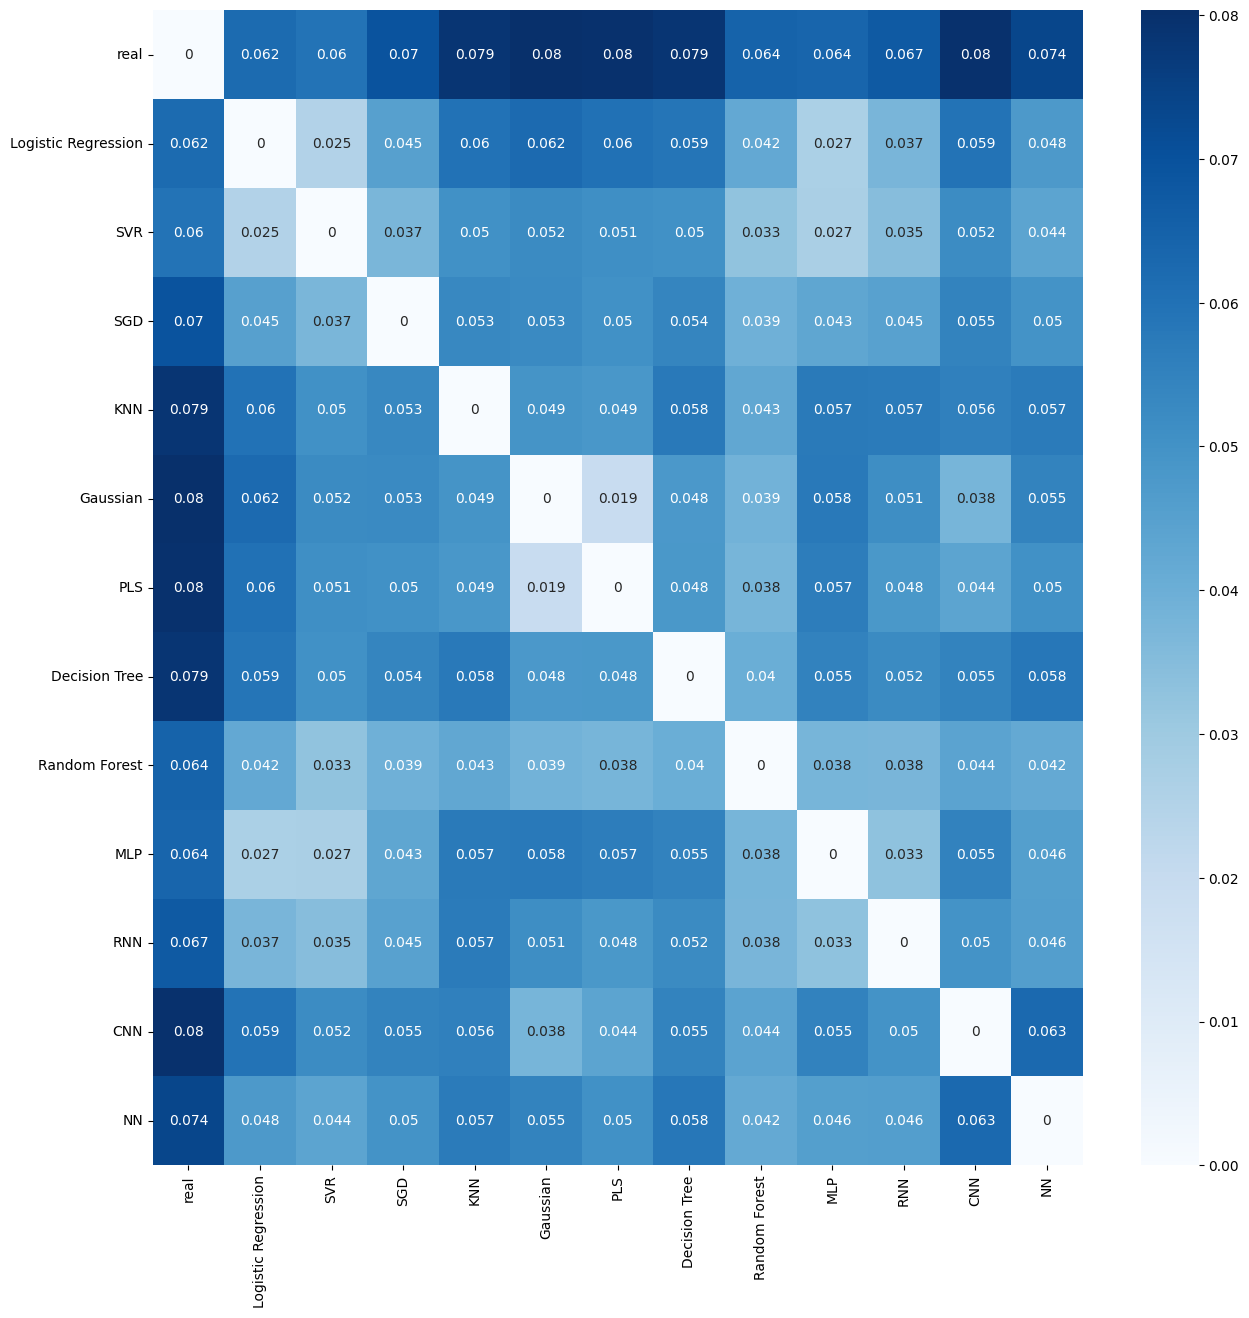
\includegraphics[width=\textwidth]{images/mae_matrix.png}
    \caption{}
    \label{mae-matrix}
\end{figure}


% Interpretation: Provide an interpretation of your findings and 
% relate them back to your research questions or hypotheses. Discuss 
% the implications of your results for the broader field of weather 
% prediction and the use of artificial intelligence and machine learning 
% techniques in this area.
\subsection{Interpretacja}

% Limitations: Discuss any limitations of your study that may 
% have affected the validity or generalizability of your findings. 
% Be sure to acknowledge any potential sources of bias or confounding variables.
\subsection{Ograniczenia}